\documentclass[40pt]{article}

% Encoding.
\usepackage{geometry}
\usepackage[T2A]{fontenc}
\usepackage[utf8]{inputenc}
\usepackage[english,russian]{babel}

% Code insertion.
\usepackage[outputdir=temp]{minted}

% Math functions.
\usepackage{amsmath}

% Image insertion.
\usepackage{svg}

% No line breaks.
\usepackage[none]{hyphenat}

% ToC hyperlinks.
\usepackage{hyperref}
\hypersetup{
	colorlinks,
	citecolor=black,
	filecolor=black,
	linkcolor=black,
	urlcolor=black
}

\title{Анализ алгоритмов}
% \author{Смирнов Александр}
\date{\today}

\begin{document}

\maketitle

% \newpage
\tableofcontents
\newpage







\section{Скорость роста длины записи коэффициентов при реализации метода Гаусса (10)}

$$\left\|b_{i j}^{r}\right\| \leq(r+1) M+r^{2}$$



\begin{itemize}
	\item $||a||$ -- длина записи числа $a$
	\item $M$ -- максимальная длина записи элементов матрицы
	\item $r$ -- ранг матрицы
	\item $||b_{ij}^r||$ -- длина записи коэффицента после $r$-й итерации
\end{itemize}


\section{Представление ''длинного'' числа в файле (массиве, списке) как числа в системе счисления по модулю $p$ ($p=1000$, если \texttt{integer} $2^{16}$, если $p=10 000 000$ \texttt{longinteger} $2^{32}$). Запись из файла. Оценка числа шагов. Вывод в файл. Оценка числа шагов (14)}


\subsection{Представление длинного числа}

Всякое целое неотрицательное число $x$ может быть представлено в $m$-ичной системе счисления (при $m \geq 2)$ в виде $x=m^{k-1} x_{0}+m^{k-2} x_{1}+\ldots m x_{k-2}+x_{k-1}.$ При этом $k$ -- длина записи $m$-ичного представления числа $x, 0 \leq x_{i} \leq m-1$ при $i=0, \ldots, k-1$

\subsection{Запись из файла}

\textbf{Оценка числа шагов:} квадратичное от длины записи исходного числа в файле количество ''шагов''.

Пусть в файле записано десятичное число, заданное словом $a_{1} \cdots a_{n}\left(0 \leq a_{i} \leq 9\right)$. Требуется представить его динамическим массивом (или списком).

Под ''шагом'' понимается одна из следуюших операций:
считывание цифры из файла, запись цифры в целочисленный массив, выделение первой цифры многозначного числа и её удаление из него, приписывание цифры в конец числа. Заметим, что эти ''шаги'' не равнозначны, т.к. последние два требуют нахождения остатка от деления на $10$, а также умножения на 10 и сложения.

\subsection{Вывод в файл}

\textbf{Оценка числа шагов:} линейное от длины записи исходного числа количество ''шагов''.

При выводе числа необходимо помнить, что в каждом элементе массива, в котором хранится многоразрядное число, записана не последовательность цифр, а число, записанное этими цифрами. Поэтому число, десятичная запись которого меньше, чем длина записи выбранного нами основания $m$, необходимо дополнить ведущими нулями.

Под ''шагом'' будем понимать одну из следующих операций: запись ''макроцифры'' в символьную переменную, сравнение длины записи ''макроцифры'' с $\|m-1\|$, дополнение строки ведущим нулём.



\section{Сложение двух ''длинных'' положительных чисел. Оценка числа шагов (17)}

\textbf{Оценка числа шагов:} общее число ''шагов'' при сложении двух неотрицательных чисел не превосходит $3\max \{A[0], B[0]\}+1$, то есть составляет $\mathrm{O}(\max \{A[0], B[0]\})$

Чтобы сложить два неотрицательных многоразрядных числа, записанных в массивы $A$ и $B$, достаточно последовательно складывать по модулю $m$ числа, записанные в $A[i], B[i]$ и $d[i]$ для $i=$ $1, \ldots, \max \{A[0], B[0]\}$, где $d[1]=0$, при $i>1, d[i]-$ это $1$ (если $A[i-1]+B[i-1]+d[i-1]>m$) или 0 в противном случае.

При подсчёте числа шагов в этом разделе под ''шагом'' понимается одна из следующих операций: вычисление $A[i-1]+B[i-1]+d[i-1]$ $\bmod m$, проверка условия $A[i-1]+B[i-1]+d[i-1]>m$ и вычисление $d[i]$


\section{Предикаты равенства и неравенств ''длинных'' положительных чисел. Оценка числа шагов (18)}

\textbf{Оценка числа шагов:} если под ''шагом'' понимать количество сравнений ''макроцифр'', то обшее число ''шагов'' такой процедуры не превосходит $A[0]$. В общем случае число ''шагов'' вычисления каждого из четырёх предикатов не превосходит $\min \{A[0], B[0]\}$.


Оценим число шагов вычисления значений предикатов $x=y$ и $x<y$ для случая, когда $A[0]=B[0]$.

Начиная со старшего разряда (то есть с $A[A[0]]$ и $B[B[0]])$ сравниваем значения чисел в $A[i]$ и $B[i]$ до тех пор, пока они совпадают. Если для некоторого $i_{0} A\left[i_{0}\right] \neq B\left[i_{0}\right]$, то $x \neq y$. Если при этом $A\left[i_{0}\right]<B\left[i_{0}\right]$, то $x<y$, если $A\left[i_{0}\right]>B\left[i_{0}\right]$, то $x>y$.


\section{Вычитание двух ''длинных'' положительных чисел. Оценка числа шагов (18)}

\textbf{Оценка числа шагов:} общее число  ''шагов'' при вычитании двух положительных чисел не превосходит $4 \max \{A[0], B[0]\}+1$, то есть составляет $\mathrm{O}(\max \{A[0], B[0]\})$.

При подсчёте числа шагов в этом разделе под ''шагом'' понимается одна из следуюшци операций: вычисление $A[i-1]-B[i-1]-d[i-1]$ $(\bmod m)$, проверка условия $A[i-1]+B[i-1]+d[i-1]>0$ и вычисление $d[i]$. Кроме того, предварительно проверяется условие $x \geq y$.




\section{Умножение ''длинного'' числа на короткое. Оценка числа шагов (19)}

\textbf{Оценка числа шагов:} общее число операций не превосходит $\max \{1,2+6 A[0]+$ $\max \{1,3\}\}=5+6 A[0]$, то есть составляет $\mathrm{O}(A[0])$.

Здесь под шагом будем понимать одну из следуюших операций: умножение макроцифр, сложение макроцифр, вычисление неполного частного и остатка от деления результата предыдущих операций на $m$. B условном операторе после else выполняется одно присваивание и оператор цикла, в котором (помимо двух операций, необходимых для организации цикла) производятся: умножение, сложение, остатка от деления на $m$, вычисление неполного частного. Всего в операторе цикла 6 ''шагов''.



\section{Умножение ''длинных'' чисел. Оценка числа шагов (20)}

\textbf{Оценка числа шагов:} В предположении, что $B[0] \leq A[0]$ (это условие проверяется за 1 «шаг» и в противном случае можно умножать $B$ на $A$), получаем оценку $O(A[0] B[0])$.


\section{Деление ''длинных'' чисел. Оценка числа шагов (21)}

\textbf{Оценка числа шагов:} $O (A[0] B[0] \cdot(A[0]-B[0]))$

Будем подбирать неполное частное от деления чисел $x$ и $y$, записанных в массивах $A$ и $B$, делением промежутка, в котором оно может находиться, пополам. Пусть $L$ и $U$ -- нижняя и верхняя границы промежутка соответственно, $M=\left\lfloor\frac{L+U}{2}\right\rfloor$ -- целая часть середины промежутка, $z=y \cdot M-$ число, которое будем сравнивать с делимым.

При этом будем предполагать, что число, записанное в $A$, больше числа, затисанного в $B$ (в противном случае неполное частное равно 0, а остаток совпадает с делимым).







\section{Оценки числа шагов метода Гауса при действиях с ''длинными'' числами}


Итоговая асимптотика: $O(\min (n, m) \cdot n m)$

При $n=m$ эта оценка превращается в $O(n^{3})$
Для длинных чисел получается $O(M*n^{3})$. 

\section{Сортировки и оценки числа их шагов: Пузырёк. Сортировка вставками. Сортировка слияниями фон Неймана (25)}

\subsection{Пузырёк}

\textbf{Сложность:} $O(n^2)$

В теле циклов сравниваются значения $a[i]$ и $a[j]$. В случае необходимости содержание элементов массива меняются местами. Обмен значениями переменных $x$ и $y$ можно осуществить с помошью трёх операторов присваивания с использованием вспомогательной переменной $z: z:=x ; x:=y ; y:=z .^{3}$ Таким образом, в теле цикла каждый раз выполняется не более четырёх операций.


\subsection{Сортировка вставками}

\textbf{Сложность:} $O(n^2)$

Элементы входной последовательности просматриваются по одному, и каждый новый поступивший элемент размещается в подходящее место среди ранее упорядоченных элементов.

\subsection{Сортировка слияниями фон Неймана}

\textbf{Сложность:} $O(n \log_{2} n)$

Сортируемый массив разбивается на две части примерно одинакового размера; Каждая из получившихся частей сортируется отдельно, например — тем же самым алгоритмом; Два упорядоченных массива половинного размера соединяются в один.


\section{Алгоритмы на графах, различные способы представления графа в компьютере (28)}


\begin{itemize}
    \item $V$ -- произвольное конечное множество; 
    \item $E$ -- подмножество множества двуэлементных подмножеств множества $V$;
    \item $G=(V, E)$ -- граф с множеством вершин $V$ и множеством рёбер $E$;
    \item $A$ -- подмножество множества упорядоченных пар множества $V$; 
    \item $G=(V, A)$ -- орграф с множеством вершин $V$ и множеством дуг $A$;
    \item $n$ -- количество вершин в графе;
    \item $m$ -- количество рёбер в графе;
    \item $N(v)$ -- окружение вершины $v$, т.е. множество вершин, смежных c $v$;
    \item $O U T(v)$ -- множество вершин орграфа, непосредственно достижимых из $v$;
    \item $I N(v)$ -- множество вершин орграфа, из которых $v$ непосредственно достижима;
    \item $\operatorname{deg}(v)$ -- степень вершины $v$, т.е. количество вершин в окружении;
    \item $w_{i j}$ -- вес ребра $\left\{v_{i}, v_{j}\right\}$ или ребра $\left(v_{i}, v_{j}\right)$ во взвешеном графе.
\end{itemize}

\subsection{Матрица смежности}

Матрица смежности графа -- это квадратная матрица $A_{n \times n},$ элементы которой определены так:
$$
a_{i j}=\left\{\begin{array}{ll}
1 & \text { если }\left\{v_{i}, v_{j}\right\} \in E \\
0 & \text { иначе }
\end{array}\right.
$$


\subsection{Списки смежности}

Списки смежности -- это одномерный массив, $i$-ым элементом которого является список вершин, смежных с $v_{i}$, т.е. окружение вершшны $v_{i}$.



\subsection{Матрица инцидентности}

Матрица инцидентности графа -- это матрица $B_{n \times m}$, элементы которой определены так:
$$
b_{i j}=\left\{\begin{array}{ll}
1 & \text { если } v_{i} \in e_{j} \\
0 & \text { иначе }
\end{array}\right.
$$

\section{Алгоритм поиска в глубину. Оценки числа шагов в зависимости от способа представления графа (28)}

\begin{itemize}
    \item \textbf{Матрица смежности: } $O\left(n^{2}\right)$
При обходе графа в глубину или в ширину для каждой вершины необходимо проверить все (при обходе в глубину - постепенно, а при обходе в ширину - сразу) вершины, смежные с данной. При использовании матрицы смежности для одной вершины это можно сделать за $n$ проверок того, следует ли помешать вершины в стек или в очередь. Эта процедура выполняется для каждой из $n$ вершин. Этим объясняется то, что алгоритмы, основанные на обходе графа в глубину или в ширину при представлении графа матрицей смежности, имеют оценку числа шагов вида $O\left(n^{2}\right)$.

Для орграфа элементы матрицы смежности определяются так
$$
a_{i j}=\left\{\begin{array}{ll}
1 & \text { если }\left(v_{i}, v_{j}\right) \in A \\
0 & \text { иначе }
\end{array}\right.
$$
Рассуждениями, аналогичными таковым для не ориентированного графа, получаем оценку числа шагов вида $O\left(n^{2}\right)$.

    \item \textbf{Списки смежности: } $O(n+m)$. Для графов с разными свойствами эта оценка может быть видоизменена.

Если граф является дереном или лесом, то $m<n$ и оценка принимает вид $O(n)$.

Ecru rpaф полный, то $m=\frac{n(n-1)}{2}$ и оценка принимает вид $O\left(n^{2}\right)$. Если степени всех вершин графа не превосходят некоторой константы $C$ (сушественно меньшей, чем $n$), то $m \leq C n$ и оценка принимает вид $O(n)$.

Если граф связен и степени вершин произвольны, то $m \geq n-1$ и оценка принимает вид $O(m)$.

Для орграфа список смежности для вершины $v$ состоит из вершин, входяших в $O U T(v)$ (или в $I N(v))$, Поскольку $\sum_{v \in V}\|O U T(v)\|=\sum_{v \in V}\|I N(v)\|=m$, то рассуждениями, аналогичными для не ориентированного графа, получаем оценку числа шагов вида $O(n+m)$.
    \item \textbf{Матрица инцидентности: } $O(n m)$
\end{itemize}




\section{Алгоритм поиска в ширину. Оценки числа шагов в зависимости от способа представления графа (28)}

\begin{itemize}
    \item \textbf{Матрица смежности: } $O\left(n^{2}\right)$
        При обходе графа в глубину или в ширину для каждой вершины необходимо проверить все (при обходе в глубину - постепенно, а при обходе в ширину - сразу) вершины, смежные с данной. При использовании матрицы смежности для одной вершины это можно сделать за $n$ проверок того, следует ли помешать вершины в стек или в очередь. Эта процедура выполняется для каждой из $n$ вершин. Этим объясняется то, что алгоритмы, основанные на обходе графа в глубину или в ширину при представлении графа матрицей смежности, имеют оценку числа шагов вида $O\left(n^{2}\right)$.

Для орграфа элементы матрицы смежности определяются так
$$
a_{i j}=\left\{\begin{array}{ll}
1 & \text { если }\left(v_{i}, v_{j}\right) \in A \\
0 & \text { иначе }
\end{array}\right.
$$
Рассуждениями, аналогичными таковым для не ориентированного графа, получаем оценку числа шагов вида $O\left(n^{2}\right)$.

    \item \textbf{Списки смежности: } $O(n+m)$. Для графов с разными свойствами эта оценка может быть видоизменена.

Если граф является дереном или лесом, то $m<n$ и оценка принимает вид $O(n)$.

Ecru rpaф полный, то $m=\frac{n(n-1)}{2}$ и оценка принимает вид $O\left(n^{2}\right)$. Если степени всех вершин графа не превосходят некоторой константы $C$ (сушественно меньшей, чем $n$), то $m \leq C n$ и оценка принимает вид $O(n)$.

Если граф связен и степени вершин произвольны, то $m \geq n-1$ и оценка принимает вид $O(m)$.

Для орграфа список смежности для вершины $v$ состоит из вершин, входяших в $O U T(v)$ (или в $I N(v))$, Поскольку $\sum_{v \in V}\|O U T(v)\|=\sum_{v \in V}\|I N(v)\|=m$, то рассуждениями, аналогичными для не ориентированного графа, получаем оценку числа шагов вида $O(n+m)$.
    \item \textbf{Матрица инцидентности: } $O(n m)$
\end{itemize}




\section{Задачи, решаемые с помощью этих алгоритмов: выделение компонент связности; проверка на двудольность и выделение долей; выделение остова графа}

\subsection{Выделение компонент связности}

Компонента связности графа $G$ -- максимальный (по включению) связный подграф графа $G$. Другими словами, это подграф $G(U)$, порождённый множеством $U \subseteq V(G)$ вершин, в котором для любой пары вершин $u, v \in U$ в графе $G$ существует $(u, v)$-цепь и для любой пары вершин $u \in U, w \notin U$ не существует $(u, w)$-цепи.

Для выделения компонент связности можно использовать поиск в ширину или поиск в глубину. При этом затраченное время будет \textbf{линейным} от суммы числа вершин и числа рёбер графа.

\subsection{Проверка на двудольность и выделение долей}

\textbf{Двудольный граф} или биграф в теории графов -- это граф, множество вершин которого можно разбить на две части таким образом, что каждое ребро графа соединяет какую-то вершину из одной части с какой-то вершиной другой части, то есть не существует рёбер между вершинами одной и той же части.

Для того, чтобы проверить граф на предмет двудольности, достаточно в каждой компоненте связности выбрать любую вершину и помечать оставшиеся вершины во время обхода графа (например, поиском в ширину) поочерёдно как чётные и нечётные. Если при этом не возникнет конфликта, все чётные вершины образуют множество $U$, а все нечётные -- $V$.

\subsection{Выделение остова графа}

\textbf{Остовное дерево графа} -- это дерево, подтраф данного графа, с тем же числом вершин, что и у исходного графа. Неформально говоря, остовное дерево получается из исходного графа удалением максимального числа рёбее, входящих в циклы, но без нарушения связности графа. остовное дерево включает в себя все $n$ вершин исходного графа и содержит $n-1$ ребро.

Остовное дерево может быть построено практически любым алгоритмом обхода графа, например поиском в глубину или поиском в ширину. Оно состоит из всех пар рёбер $(u, v)$, таких, что алгоритм, просматривая вершину $u$, обнаруживает в её списке смежности новую, не обнаруженную ранее вершину $v$.



\section{Нахождение остова минимального веса. Метод Р. Прима. Оценки числа шагов (32)}

Оценки числа шагов работы этого алгоритма аналогичны оценкам числа шагов алгоритма Дейкстры за исключением того, что в п. 4 не выполняется операция сложения. В результате получаем
$$ O\left(n^{2}+m\right)=O\left(n^{2}\right) $$



\section{Алгоритм Дейкстры поиска кратчайшего пути. Оценки числа шагов (31)}

\textbf{Сложность: } $O(n^2 + m) = O(n^2)$

Задан взвешенный орграф $G=(V, A)$ (все веса $w_{i j}$ положительны) и две выделенные вершины $s$ -- старт и $f$ -- финиш. Требуется найти кратчайший путь из $s$ в $f$.


\section{Нахождение циклов и мостов в графе. Оценки числа шагов}

\subsection{Циклы}

\textbf{Замкнутый обход} состоит из последовательности вершин, начинающейся и заканчивающейся в той же самой вершине, и каждые две последовательные вершины в последовательности смежны.

\textbf{Сложность: } $O(n + m)$

Неориентированный граф имеет цикл в том и только в том случае, когда поиск в глубину (DFS) находит ребро, которое приводит к уже посещённой вершине (обратная дуга). Таким же образом, все обратные рёбра, которые алгоритм DFS обнаруживает, являются частями циклов. Для неориентированных графов требуется только время $O(n)$ для нахождения цикла в графе с $n$ вершинами, поскольку максимум $n-1$ рёбер могут быть рёбрами дерева.

\subsection{Мосты}

\textbf{Мост} -- ребро в теории графов, удаление которого увеличивает число компонент связности. Эквивалентное определение -- ребро является \textbf{мостом} в том и только в том случае, если оно не содержится ни в одном цикле.

\textbf{Сложность: } $O(n + m)$

\section{Эйлеров цикл.  Оценки числа шагов}

\textbf{Эйлеров путь} -- это путь в графе, проходящий через все его рёбра.

\textbf{Эйлеров цикл} -- это эйлеров путь, являющийся циклом.

Граф называется эйлеровым, если он содержит эйлеров цикл.
Мультиграф - граф, в котором разрешается присутствие кратных рёбер.
Асимптотика задачи поиска эйлерова пути $\mathrm{O}(\mathrm{m})$ при использовании списков смежности.


\section{Гамильтонов цикл.  Оценки числа шагов (33)}

\textbf{Гамильтонов цикл} -- цикл , который проходит через каждую вершину данного графа ровно по одному разу.

\textbf{Гамильтонов граф} -- граф, содержащий гамильтонов цикл.

Асимптотика задачи нахождения гамильтонова цикла в графе $\mathrm{O}\left(\mathrm{d}^{\wedge}(\mathrm{n}-1)\right)$. Где $\mathrm{d}$ это максимальная степень вершины в графе - $1 .$

\section{Алгоритм генерации всех независимых множеств.  Оценки числа шагов (не будут спрашивать)}

\section{Теорема о НМ, ВП, КЛИКА.  Оценки числа шагов (34)}

Алгоритм для поиска клик подойдет для поиска НМ. Ищем клики в $G$ (дополнение), в $G$ это будут независимые множества Алгоритм Брона-Кербоша -- метод ветвей и границ для поиска всех клик. Вычислительная сложность алгоритма линейна относительно количества клик в графе. В худшем случае алгоритм работает за $О(3^{n/3})$ шагов.

    \begin{figure}[h!]
        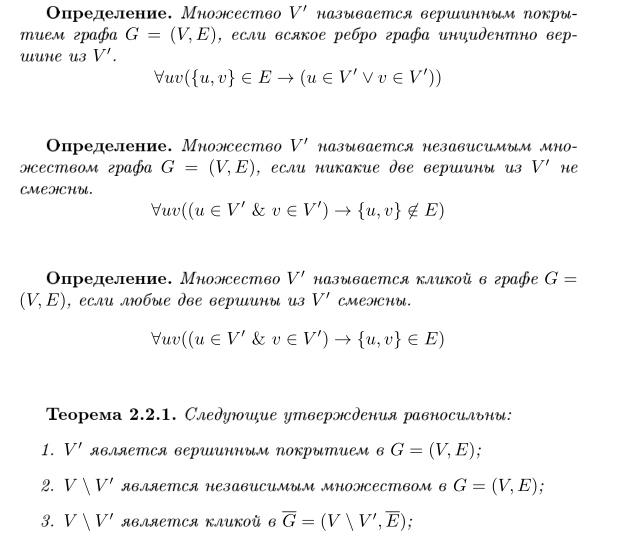
\includegraphics[width=1\textwidth]{./images/21.png}
        \centering
    \end{figure}

\section{Отличия между интуитивным и математическим понятиями алгоритма}
(ИНТУИТИВНОЕ ОПРЕДЕЛЕНИЕ)
Первые попытки дать математическое определение алгоритма
привели приблизительно к следующим требованиям:
\begin{itemize}
    \item Определенность данных: вид исходных данных строго определен.
    \item Дискретность: процесс разбивается на отдельные шаги.
    \item Детерминированность: результат каждого шага строго определјн в зависимости от данных, к которым он применен
    \item Элементарность шага: переход на один шаг прост.
    \item Направленность: что считать результатом работы алгоритма,
если следующий шаг невозможен.
    \item Массовость: множество возможных исходных данных потенциально бесконечно
\end{itemize}

Первыми математическими понятиями
алгоритма были рекурсивные функции и машины Тьюринга.

\textbf{Определение.} Простейшими называются функции натурального аргумента S, O, ${I_m}^n$, определяемые равенствами: S(x) = x + 1,
O(x) = 0, ${I_m}^n(x_1, . . . , x_n) = x_m$ при $1 \leq m \leq n$.

\textbf{Определение.} Функция f от n + 1 переменных получена из
функции g от n переменных и функции h от n + 2 переменных с
помощью оператора примитивной рекурсии, если 

$\left\{\begin{aligned}
f\left(x_{1}, \ldots, x_{n}, 0\right) &=g\left(x_{1}, \ldots, x_{n}\right) \\
f\left(x_{1}, \ldots, x_{n}, y+1\right) &=h\left(x_{1}, \ldots, x_{n}, y, f\left(x_{1}, \ldots, x_{n}, y\right)\right)
\end{aligned}\right.$

\textbf{Определение.} Функция называется примитивно рекурсивной, если она может быть получена из простейших с помощью
применения операторов подстановки и/или примитивной рекурсии.

\textbf{Определение.} Функция называется частично рекурсивной,
если она может быть получена из простейших с помощью применения операторов подстановки, примитивной рекурсии и/или $\mu$-оператора.

\textbf{Определение.} Функция называется общерекурсивной, если
она может быть получена из простейших с помощью применения
операторов подстановки, примитивной рекурсии и/или обобщенного µ-оператора.

\section{Машины Тьюринга и их модификации. Тезис Тьюринга-Чёрча}

Машины Тьюринга, основные определения, стр. 40-41

\textbf{Тезис Тьюринга-Черча} Всякая интуитивно вычислимая функция может быть вычислена на машине Тьюринга.

Модификации машин Тьюринга --- стр. 45-47

\section{Теорема о числе шагов МТ, моделирующей работу k-ленточной МТ}

\textbf{Теорема.} По всякой k-ленточной машине Тьюринга MTk,
заканчивающей работу с исходными данными X за t шагов, можно
построить одноленточную машину Тьюринга MT1, результат работы которой с исходными данными X совпадает с результатом
работы исходной и число шагов которой составляет $O(t^2)$.

\section{Недетерминированные МТ.  Теорема о числе шагов МТ, моделирующей работу недетерминированной МТ}

Недетерминированные машины Тьюринга часто используются
для проверки истинности утверждений типа $\exists Y P(X, Y )$ (существует такой объект Y , для которого справедливо утверждение P(X, Y )).
Для проверки истинности таких утверждений работу недетерминированной машины Тьюринга можно разбить на два этапа:
\begin{itemize}
    \item этап угадывания, при реализации которого лента в недетерминированном режиме размножается, и на каждой из них выписывается ѕпретендентї на решение;
    \item этап проверки, при реализации которого машина работает в
детерминированном режиме и проверяет конкретного "претендента"
на то, является ли он решением
\end{itemize}

\textbf{Теорема.} По всякой недетерминированной машине Тьюринга, проверяющей предикат $\exists P(X, Y )$ и заканчивающей работу с
исходными данными X за t шагов, можно построить одноленточ-
ную машину Тьюринга, результат работы которой с исходными
данными X совпадает с результатом работы исходной и число шагов которой составляет $2^{O(t)}$

\section{Понятия сложности алгоритма от данных, сложность алгоритма, сложность задачи. Верхняя и нижняя оценки сложности}

Под вычислительной сложностью алгоритма понимают функцию, зависящую от ДЛИНЫ записи исходных данных и характеризующую
\begin{itemize}
    \item число шагов работы алгоритма над исходными данными (временная сложность);
    \item объем памяти, необходимой для работы алгоритма над исходными данными (емкостная или зональная сложность).
\end{itemize} 

\textbf{Определение.} Сложностью $S_A(P)$ алгоритма A при работе
над данными P называется число шагов или объем памяти, затра-
ченные в процессе работы алгоритма A над данными P.

\textbf{Определение.} Верхней (нижней) оценкой сложности алгоритма A при работе над данными длины n называется $S_{A}^{U}(n)=\max _{P:\|P\|=n}\left\{S_{A}(P)\right\}$
\section{Соотношение между временем работы алгоритма требуемой памятью}
\section{Классы алгоритмов и задач. Схема обозначений}

$\begin{array}{|c|c|c|c|}
\hline \begin{array}{c}
\text { Класс } \\
\text { функций или } \\
\text { предикатов }
\end{array} & \begin{array}{c}
\text { Детерминирован- } \\
\text { ная или неде- } \\
\text { терминированная }
\end{array} & \begin{array}{c}
\text { Функция } \\
\text { сложности }
\end{array} & \begin{array}{c}
\text { Временнáя } \\
\text { или } \\
\text { ёмкостная }
\end{array} \\
\hline \mathrm{F} & {[\mathrm{D}]} & \text { LOG } & {[\mathrm{TIME}]} \\
& \mathrm{N} & \text { LIN } & \text { SPACE } \\
& & \text { QLIN } & \\
& & \mathrm{P} \text { (Poly) } & \\
& & \text { EXP-LIN } & \\
& & \text { EXP } & \\
& & \vdots & \\
\hline
\end{array}$

\textbf{Определение.} Функция сложности это функция от длины записи исходных данных, ограничивающая число шагов или количество ячеек соответствующей машины Тьюринга.
\section{Классы $P$, $NP$ и $P-SPACE$. Соотношения между этими классами}

\textbf{Определение.} Класс P это класс предикатов, для которых существует алгоритм, который может быть реализован на детерминированной машине Тьюринга, число шагов которой не превосходит полинома
от длины записи исходных данных.

\textbf{Определение.} Класс NP это класс предикатов, для которых существует алгоритм, который может быть реализован на недетерминированной машине Тьюринга, число шагов которой не превосходит полинома
от длины записи исходных данных.

\textbf{Определение.} Класс P-SPACE это класс предикатов, для которых существует алгоритм, который может быть реализован на детерминированной машине Тьюринга, число использованных ячеек которой
не превосходит полинома от длины записи исходных данных.

$P \subseteq NP \subseteq P-SPACE \subseteq EXP$

\textbf{Теорема.} Если предикат вида $\exists Y P(X, Y )$ принадлежит классу
NP, то существует проверяющая его одноленточная машина Тьюринга, число шагов которой составляет $2^{p(n)}$, где p(n) полином от длины записи исходных данных $n = size(X)$.

\section{Полиномиальная сводимость и полиномиальная эквивалентность}

\textbf{Определение.} Определение. Задача $Z_{1}$ вида $\exists Y P_{1}(X, Y)$ при $X \in D_{1}$ полиномиалъно сводится к задаче $Z_{2}$ вида $\exists Y P_{2}(X, Y)$ при $X \in D_{2}$
$$
Z_{1} \propto Z_{2}
$$
если сушествует функиия $f,$ отображающая $D_{1}$ в $D_{2}$ и такая, что
\begin{itemize}
    \item существует машина Тьюринга, вычисляющая функцию f не болеечем за полиномиальное от длиньи записи исходных данных число шагов $(f \in \mathbf{F P})$
    \item задача $Z_{1}$ имеет решение с исходными данными $X$ тогда и только тогда, когда задача $Z_{2}$ имеет решение с исходными данными $f(X)$
$$
\forall X_{\in D_{1}}\left(\exists Y P_{1}(X, Y) \leftrightarrow \exists Y P_{2}(f(X), Y)\right)
$$
\end{itemize}


 \textbf{Определение.} Задача  $Z_{1} \text { полиномиально эквивалентна задаче } Z_{2}
\left(Z_{1} \sim_{p} Z_{2}\right), \text { ecли } Z_{1} \propto Z_{2} \text { и } Z_{2} \propto Z_{1}$

\section{Полиномиальная сводимость задачи ГЦ к задаче КОМИВОЯЖЁР (стр. 80)}


\section{Классы эквивалентности по отношению полиномиальной эквивалентности. Класс P – пример такого класса (стр. 81-82)}
\section{NP-полные задачи. Класс NP-полных задач — класс эквивалентности по отношению полиномиальной эквивалентности (стр. 81-82)}
\section{Задача ВЫПОЛНИМОСТЬ (ВЫП).Теорема Кука}

Дано: $U = \left\{u_1, ..., u_n\right\}$ множество пропозициональных переменных,

$C = \left\{c1, ..., cm\right\}$ множество предложений над U.

Вопрос: выполнимо ли множество C, т.е. существует ли набор значений
для переменных из U, для которого истинны все предложения из C?

$\exists u1, ..., un(c1 \& ... \& cm)$

\textbf{Теорема.} Задача ВЫП NP-полна.


\section{Задача 3-ВЫПОЛНИМОСТЬ (3-ВЫП). Её NP-полнота (84)}

\par Пусть U - множество пропозициональных переменных. C - множество предложений над U, где каждое из них состоит из трех переменных. Требуестя определить, существует ли такой набор значений переменных, что $c_1\&...\&c_m$ выполнимо.

\section{Задачи ВЕРШИННОЕ ПОКРЫТИЕ (ВП), НЕЗАВИСИМОЕ МНОЖЕСТВО (НМ), КЛИКА.  NP-полнота задачи ВП.  Полиномиальная эквивалентность этих трёх задач (85-86)}

 \par \textbf{Определение вершинного покрытия} -- множество вершин такое, что для каждого ребра из заданного графа хотя бы один из его концов содержится в этом множестве.
 
   \par \textbf{Определение клики} Клика - полный подграф исходного графа
 
   \par \textbf{Определение независимого множества} Независимое множество -- подмножество вершин графа такое, что для между любой парой вершин из этого множества нет ребра в исходном графе.
 
   \par \textbf{Вершинное покрытие} Дан граф и число k, требуется узнать есть ли в графе вершинное покрытие не более чем из k элементов. 
 
   \par \textbf{Клика} Дан граф и число k, требуется узнать есть ли в графе клика не менее чем из k вершин. 
 
   \par \textbf{Независимое множество} Дан граф и число k, требуется узнать есть ли в графе Независимое множество не менее чем из k элементов.
   
\section{NP-полнота задач ГЦ и ГП (без доказательства)}

\par Гамильтонов цикл -- NP трудная задача как и Гамильтонов путь.

\section{NP-полнота задач 3-С и РАЗБИЕНИЕ (без доказательства) }

\par \textbf{Задача 3-C (трехмерное сочетание):} Дано множество $M = X \times Y \times Z$. X,Y,Z - попарно не пересекающиеся множества мощности $q$. Требуется узнать существует ли подмножество $M' \in M$ мощности q, такое, что у никаких двух элементов из этого множества значения хотя бы по одной из координат совпадают.
 
 
    \par \textbf{Задача Разбиение:} Дано множество $A$, для каждого $a \in A$ задан вес $s(a)$ -- целое положительное число.
    Требуется разбить исходное множество на два подмножества одинакого веса.
    
    
\section{Метод сужения доказательства NP-полноты (89-90)}


\par \textbf{Определение} Задача $Z_1$ называется сужением на множество $D_1$ задачи $Z_2$ с исходными данными из множества $D_2$, если $D_1$ содержится в $D_2$ и $\forall X(X\in) D_1 \rightarrow (Z_1 \leftrightarrow Z_2)$ 
 
	\par \textbf{Метод сужения:} Чтобы доказать NP-полноту задачи $Z$ достаточно доказать, что $Z \in NP$ и что среди известных NP-полных задач найти такую задачу $Z_1$, что она является сужением задачи $Z$
	
\section{«Похожие» задачи и их сложность}

Этого говна не будет

\section{Анализ подзадач (90-91)}

\par \textbf{Определение} Задача $Z_1$ с исходными данными $D_1$ является подзадачей $Z_2$ с исходными данными из множества $D_2$, если $D_1$ содержится в $D_2$ и $\forall X(X\in) D_1 \rightarrow (Z_1 \leftrightarrow Z_2)$ 
 
     \par Например 3-SAT задача подзадача SAT задачи.
     
\section{Алгоритм решения задачи РАЗБИЕНИЕ}

\par \textbf{Решение 1:} Общая идея: рекурсия. Подсчитаем сумму всего массива -- если она нечетная, то задачу не решить. Если она четная, то ок -- решаем рекурсивно. Каждый элемент может быть отнесен к одному из двух множеств. Попробуем решить задачу, нахождения множества с суммой равной половине исходной. Для этого рекурсивно будем считать достигается ли эта сумма, если выкинуть или не выкидывать последний элемент из текущего множества. Асимптотика -- $\mathcal O(n2^n)$
    \par \textbf{Решение 2:} Воспользуемся методом динамического программирования. 
    \par Пусть $dp[i][j]$ -- ответ на вопрос: правда ли, что сумма на j-ом префиксе равна i? (0/1 = да/нет)
    \par Пересчет дп -- $\mathcal O(n*sum )$, что может быть долго, если сумма достаточно большая.

\section{Задачи с числовыми параметрами. Псевдополиномиальные задачи (92)}

 \textbf{Определение.} Задача с числовыми параметрами называется псевдополиномиальной, если число шагов решающей еј машины Тьюринга не
превосходит полинома от этих числовых параметров и длины записи
остальных исходных данных.
 
    \par Казалось бы алгоритм задачи разбиение, использующий метод динамического программирования, работает за полином, но из-за скорости роста данных он на самом деле Псевдополиномиальный

\end{document}